\documentclass[border=4pt]{standalone}
\usepackage[T1]{fontenc}
\usepackage{helvet}
\renewcommand{\familydefault}{\sfdefault}
\usepackage{graphicx}
\usepackage{caption}
\usepackage{amsmath}
\captionsetup{font={sf,footnotesize},labelfont={sf,bf,footnotesize},justification=justified,singlelinecheck=false}
\begin{document}
\setcounter{figure}{11}
\begin{minipage}{7.20in}
\centering
\begin{figure}[htbp]
    \centering
    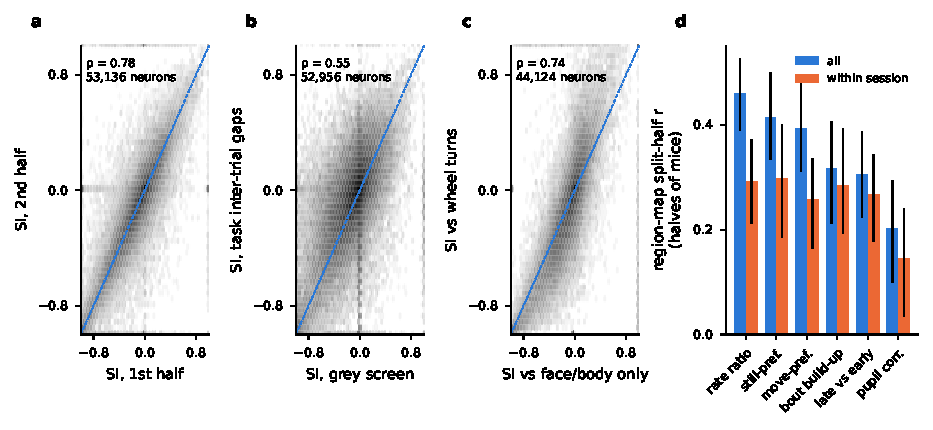
\includegraphics[width=\linewidth]{fig12_still_stability_panels.pdf}
    \caption{Stillness preference is reproducible within recordings; region differences are reproducible but modest. \textbf{a} Stillness index SI = (still $-$ moving)/(still $+$ moving) of each neuron in the first vs second half of the grey screen. \textbf{b} SI on the grey screen vs in the inter-trial gaps of the task, a second behavioural context recorded earlier in the session. \textbf{c} SI computed against face/body movements without wheel turns vs against wheel turns. \textbf{d} Reliability of region maps over animals: Spearman r between region means from two random halves of the mice (200 splits, median and 5--95\% range), from raw neuron values (blue) and after subtracting each session's mean (orange). Regions with $\geq$20 neurons from $\geq$3 mice. Region within session explains 13\% of neuron variance in the rate ratio (label shuffle 4\%), session 6\%.}
    \label{fig:stability}
\end{figure}
\end{minipage}
\end{document}
